%=========================================================
% Capítulo 6 — Formulação estatística da assimilação de dados
%=========================================================
\chapter{Formulação estatística da assimilação de dados}
\label{ch:formulacao-estatistica}

\noindent\textbf{Resumo:}
Neste capítulo, apresentamos a base estatística da assimilação de dados.  
A assimilação é vista como uma estimativa ótima que combina informações de um modelo (background) e observações (dados), ponderadas pelos respectivos erros.  
Mostra-se que o problema é equivalente ao dos mínimos quadrados ponderados, conduzindo à equação clássica da análise e ao ganho de Kalman.

%---------------------------------------------------------
\section{Motivação estatística}
Toda medição contém incerteza.  
Do mesmo modo, todo modelo numérico é uma representação aproximada da realidade.  
A assimilação de dados reconhece explicitamente essas imperfeições e procura combinar as fontes de informação de modo a minimizar o erro médio quadrático.

Denotemos:
\begin{itemize}
  \item $\mathbf{x}_b$ — vetor de \textbf{background} (ou previsão de curto prazo);
  \item $\mathbf{y}$ — vetor de \textbf{observações};
  \item $\mathbf{H}$ — operador que transforma o estado do modelo em espaço de observação;
  \item $\mathbf{x}_a$ — vetor \textbf{analisado} (resultado da assimilação).
\end{itemize}

O problema é então formular uma estimativa $\mathbf{x}_a$ que combine coerentemente as duas fontes:
\begin{equation}
\mathbf{x}_a = \mathbf{x}_b + \mathbf{K}\,(\mathbf{y} - \mathbf{H}\mathbf{x}_b),
\label{eq:analysis}
\end{equation}
onde $\mathbf{K}$ é a \emph{matriz de ganho} (ou matriz de ponderação ótima).

%---------------------------------------------------------
\section{Matriz de covariância e erro}
Seja o erro de background $\boldsymbol{\epsilon}_b = \mathbf{x}_b - \mathbf{x}_t$, onde $\mathbf{x}_t$ é o estado verdadeiro desconhecido.  
A matriz de covariância associada é:
\[
\mathbf{B} = \mathrm{E}[\boldsymbol{\epsilon}_b \boldsymbol{\epsilon}_b^\top].
\]
De forma análoga, o erro de observação $\boldsymbol{\epsilon}_o = \mathbf{y} - \mathbf{H}\mathbf{x}_t$ possui covariância:
\[
\mathbf{R} = \mathrm{E}[\boldsymbol{\epsilon}_o \boldsymbol{\epsilon}_o^\top].
\]
Essas matrizes representam o \emph{grau de confiança} nas fontes de informação.  
Valores pequenos em $\mathbf{R}$ indicam observações precisas; valores grandes em $\mathbf{B}$ indicam grande incerteza no modelo.

%---------------------------------------------------------
\section{Função custo e mínimos quadrados ponderados}
A análise é obtida minimizando a função custo:
\begin{equation}
J(\mathbf{x}) = (\mathbf{x} - \mathbf{x}_b)^\top \mathbf{B}^{-1} (\mathbf{x} - \mathbf{x}_b)
+ (\mathbf{y} - \mathbf{H}\mathbf{x})^\top \mathbf{R}^{-1} (\mathbf{y} - \mathbf{H}\mathbf{x}).
\label{eq:Jstat}
\end{equation}
O primeiro termo mede o desvio em relação ao modelo, ponderado por $\mathbf{B}^{-1}$, e o segundo, o desvio em relação às observações, ponderado por $\mathbf{R}^{-1}$.  
A minimização de \eqref{eq:Jstat} é análoga ao problema de mínimos quadrados com pesos.

Derivando $J$ em relação a $\mathbf{x}$ e igualando a zero:
\[
\frac{\partial J}{\partial \mathbf{x}} = 2\mathbf{B}^{-1}(\mathbf{x}-\mathbf{x}_b)
- 2\mathbf{H}^\top \mathbf{R}^{-1}(\mathbf{y}-\mathbf{H}\mathbf{x}) = 0,
\]
obtemos:
\[
(\mathbf{B}^{-1} + \mathbf{H}^\top \mathbf{R}^{-1}\mathbf{H})\mathbf{x}_a
= \mathbf{B}^{-1}\mathbf{x}_b + \mathbf{H}^\top \mathbf{R}^{-1}\mathbf{y}.
\]
A solução, após manipulação algébrica, conduz à forma clássica:
\begin{equation}
\boxed{\mathbf{x}_a = \mathbf{x}_b + \mathbf{K}(\mathbf{y} - \mathbf{H}\mathbf{x}_b),}
\label{eq:xa-final}
\end{equation}
onde
\begin{equation}
\boxed{\mathbf{K} = \mathbf{B}\mathbf{H}^\top (\mathbf{H}\mathbf{B}\mathbf{H}^\top + \mathbf{R})^{-1}.}
\label{eq:kalman-gain}
\end{equation}

%---------------------------------------------------------
\section{Interpretação do ganho de Kalman}
A matriz $\mathbf{K}$ define quanto da inovação $(\mathbf{y}-\mathbf{H}\mathbf{x}_b)$ deve ser aplicada para corrigir o background.  
Se as observações são muito confiáveis ($\mathbf{R}$ pequeno), $\mathbf{K}$ se aproxima de $\mathbf{H}^{-1}$, e a análise tende às observações.  
Se o modelo é mais confiável ($\mathbf{B}$ pequeno), $\mathbf{K}$ tende a zero, e a análise permanece próxima do background.

A equação \eqref{eq:kalman-gain} mostra explicitamente a ponderação por erro — o mesmo princípio intuitivo que vimos no exemplo unidimensional no Capítulo~\ref{ch:interpolacao}:
\[
T_a = \frac{T_m/\sigma_m^2 + T_o/\sigma_o^2}{1/\sigma_m^2 + 1/\sigma_o^2}.
\]

%---------------------------------------------------------
\section{Resposta do filtro e propagação de erro}
O ganho $\mathbf{K}$ atua como um filtro espacial e estatístico.  
Aplicado a uma sequência de atualizações, ele controla quanto das estruturas observadas é incorporado e quanto do ruído é atenuado.  
A covariância do erro de análise é:
\begin{equation}
\mathbf{A} = (\mathbf{I} - \mathbf{K}\mathbf{H})\,\mathbf{B}.
\label{eq:cov-analysis}
\end{equation}
Essa expressão mostra que o erro de análise é sempre menor (ou igual) ao erro de background, refletindo a melhoria obtida pela assimilação.

\begin{figure}[h!]
\centering
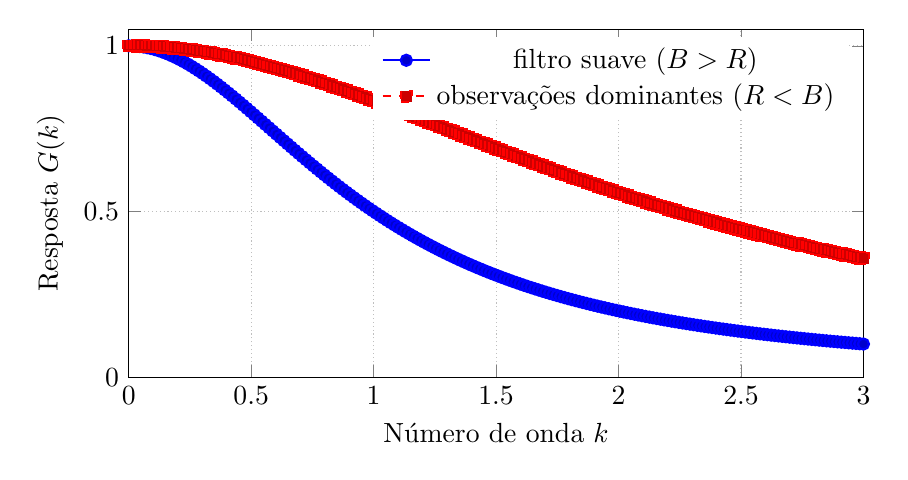
\begin{tikzpicture}
\begin{axis}[
  width=0.9\linewidth, height=6cm,
  xlabel={Número de onda $k$}, ylabel={Resposta $G(k)$},
  xmin=0, xmax=3, ymin=0, ymax=1.05,
  grid=both, grid style={densely dotted},
  legend style={at={(0.98,0.98)},anchor=north east,draw=none}
]
  \addplot+[domain=0:3, samples=200, thick] {1/(1 + x^2)}; \addlegendentry{filtro suave ($B>R$)}
  \addplot+[domain=0:3, samples=200, thick, dashed] {1/(1 + 0.2*x^2)}; \addlegendentry{observações dominantes ($R<B$)}
\end{axis}
\end{tikzpicture}
\caption{Resposta espectral do filtro de assimilação: o ganho $\mathbf{K}$ atua como um filtro passa-baixa, ponderando a contribuição das observações conforme a escala espacial.}
\label{fig:kalman-filter-response}
\end{figure}

%---------------------------------------------------------
\section{Síntese e ligação com os métodos anteriores}
O formalismo apresentado neste capítulo demonstra que a assimilação de dados é uma generalização estatística dos métodos de análise objetiva.  
Os pesos empíricos de Cressman e Barnes são substituídos por ponderações ótimas derivadas das matrizes $\mathbf{B}$ e $\mathbf{R}$.  
A iteração sucessiva dá lugar à atualização analítica por meio da matriz de ganho.  
Em essência, a assimilação moderna é uma \emph{interpolação ótima ponderada pelos erros estatísticos}, uma fusão entre física, estatística e computação.

No próximo capítulo, veremos como esse formalismo pode ser aplicado de forma dinâmica — com a atualização contínua do estado e da covariância — culminando no \emph{Filtro de Kalman} e em suas extensões para sistemas não lineares.

% Fim do Capítulo 6
